\section[GPS的计算模型]{GPS的计算模型\\Computational Models for GPS}
在研究综合性强、相当复杂的实时动态定位(RTK)数据处理的代码之前,估计仅利用伪距观测值获得的精度以及利用相位观测值获得的改进是合理的。第九章介绍了只利用伪距观测值描述和研究定位的方法。利用这种方式,大多数人了解了GPS 的有效性,它是一种简单的手持接收机的形式。

我们利用接收机i上的L1频率对卫星k的单程码观测值进行处理:
$$
Pseudorange  \hspace{1cm} P_{1,i}^{k}=\rho_{i}^{k}+T_{i}^{k}+I_{i}^{k}+noise.
$$

C/A码观测值的标准偏差为 $\sigma_{code}$,同时当一台接收机追踪至少4 颗卫星时,单点定位的标准偏差为 $\sigma \approx$。利用SBAS时,单台接收机的标准偏差可以达到 $\sigma \approx$。

在easy4中对两台接收机接收到的L1载波上的码观测值作单差:
$$
P_{1}=P_{1,i}^{k}-P_{1,j}^{k}
$$

利用这种方法在精度提高上没有的效果。事实上,还会造成精度的损失。

性能上的巨大改变是通过观测P码和信号的相位实现的,这一改变也影响着价格。手持式接收机需要100美元,而组合码和相位双频接收机需要20000美元。

当加入相位观测值之后,P码观测值的标准偏差由$\sigma_{code}$减小到$\sigma_{phase}$,100倍的改进是很明显和重要的。载波相位观测方程为:
$$
Carrier phase  \hspace{1cm} \Phi_{1,i}^{k}=\rho_{i}^{k}+T_{i}^{k}-I_{i}^{k}+\lambda_{1}N_{1}+ clock errors + multipath + noise
$$

L1载波上的单差相位观测方程为
$$
\Phi_{1}=\Phi_{1,i}^{k}-\Phi_{1,j}^{k}
$$

最后,我们对卫星k,l作双差,双差P码观测方程为:
$$
P_{1,ij}^{kl}=(P_{1,i}^{k}-P_{1,i}^{l})-(P_{1,j}^{k}-P_{1,j}^{l})+noise
$$

对流层延迟可以通过模型计算,接收机钟差被消除,卫星钟差可以被计算出来,噪声只有电离层的影响,则
$$
P_{1,ij}^{kl}=(\rho_{i}^{k}-\rho_{i}^{l})-(\rho_{j}^{k}-\rho_{j}^{l})+I_{ij}^{kl}
$$

对于相位观测值$\Phi$,观测方程包含整周模糊度如下:
$$
\Phi_{1,ij}^{kl}=(\rho_{i}^{k}-\rho_{i}^{l})-(\rho_{j}^{k}-\rho_{j}^{l})-I_{ij}^{kl}+\lambda_{1}((N_{1,i}^{k}-N_{1,i}^{l})-(N_{1,j}^{k}-N_{1,j}^{l}))+noise
$$

使用码观测值,相位观测值以及固定模糊度的精密差分定位的标准差可以达到$\sigma \approx$。

\subsection{10.4.1 差分GPS}

差分GPS是以坐标已知的站为基础的,根据基准站计算距离改正值。这些改正值被传送给一个或者更多的移动接收机上以提高位置精度,见图10.4。利用邻近的两个站i、j重述差分定位(DGPS)的定义:\\
- 基线距离满足$I_{i}^{k}=I_{j}^{k}$ 和$T_{i}^{k}=T_{j}^{k}$。\\
- 基准站i的坐标是已知的。\\
- 站i和j的x坐标的差值向量是未知的。\\
- 我们只考虑每个历元的L1观测值,除非另有说明。

以下内容和实例解释了差分GPS的不同模型。

\subsection{10.4.2 DGPS:相位观测值}

重新建立接收机i,卫星k在载波L1上的相位观测方程:
\begin{equation}
	\Phi_{i}^{k}=\rho_{i}^{k}+cdt_{i}-cdt^{k}-I_{i}^{k}+T_{i}^{k}+\lambda_{1}N_{i}^{k}-\epsilon_{i}^{k}
\end{equation}

大气延迟和卫星钟差组合成如下:
\begin{equation}
	E_{i}^{k}=cdt^{k}+I_{i}^{k}-T_{i}^{k}
\end{equation}

然后线性化,得到接收机i,j之间的单程相位方程:
$$
\Phi_{i}^{k}= cdt_{i}-E_{i}^{k}+\lambda_{1}N_{i}^{k}-\epsilon_{i}^{k}
$$
$$
\Phi_{j}^{k}= -(u_{j}^{k})^{T}x_{j}+cdt_{j}-E_{j}^{k}+\lambda_{1}N_{j}^{k}-\epsilon_{j}^{k}
$$

此处
\begin{equation}
	-(u_{j}^{k})^{T}=(\frac{X_{ECEF}^{k}-X_{i}}{\rho_{i}^{k}},\frac{Y_{ECEF}^{k}-Y_{i}}{\rho_{i}^{k}},\frac{Z_{ECEF}^{k}-Z_{i}}{\rho_{i}^{k}})
\end{equation}

\subsection{10.4.3 DGPS:站际单差}

假设接收机i的位置是已知的,$P_{i}^{k}$与基准接收机的钟差$cdt_{i}$ 相关且可以被应用到移动站(接收机j) $P_{j}^{k}$的距离改正中。差分GPS的原理即为对接收机i、j观测模型的组合,利用卫星k=1到k=m获得基准站的准确伪距$(P_{i}^{k})^{0}$。
$$
\begin{bmatrix}
(P_{j \ obs}^{1}-(P_{j}^{1})^{0})-(P_{i \ obs}^{1}-(P_{i}^{1})^{0})\\
(P_{j \ obs}^{2}-(P_{j}^{2})^{0})-(P_{i \ obs}^{2}-(P_{i}^{2})^{0})\\
\vdots \\
(P_{j \ obs}^{m}-(P_{j}^{m})^{0})-(P_{i \ obs}^{m}-(P_{i}^{m})^{0})\\
\end{bmatrix}
=
\begin{bmatrix}
-(u_{j}^{1})^{0}&1\\
-(u_{j}^{2})^{0}&1\\
\vdots \\
-(u_{j}^{m})^{0}&1\\
\end{bmatrix}
\begin{bmatrix}
x_{j}\\y_{j}\\z_{j}\\cdt_{ij}
\end{bmatrix}
$$
其中,$cdt_{j}-cdt_{i}$为接收机钟差的差值。

例10.2我们有m-1个单频码观测方程:
$$
\begin{bmatrix}
P_{ij}^{k2}\\
P_{ij}^{k3}\\
\vdots \\
P_{ij}^{km}
\end{bmatrix}
=\begin{bmatrix}
-(u_{j}^{k2})\\
-(u_{j}^{k3})\\
\vdots \\
-(u_{j}^{km})
\end{bmatrix}
x_{j}.
$$\\
4颗卫星(3个双差方程)求解得到$x_{j}$的三个分量。

比较当前的码观测方程和例10.4中的相位观测方程,我们可以得到相位观测方程中所有模糊度在形式上都设置为零。

\begin{figure}
	\centering
	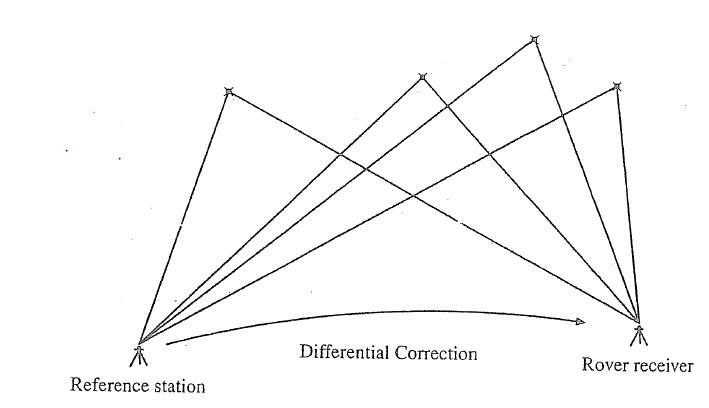
\includegraphics[width=0.4\linewidth]{TeX_files/Part03/chapter10/image/9-4}
	\caption{差分GPS原理:基准站位置已知}
	\label{fig:9-4}
\end{figure}

\subsection{10.4.4 DGPS:站际星际双差}

对已做单差(接收机之间)的卫星k和l作差,卫星k是参考卫星:
\begin{equation}
	\Phi_{ij}^{kl}=(\Phi_{j}^{l}-\Phi_{j}^{k})-(\Phi_{i}^{l}-\Phi_{i}^{k})
\end{equation}\\
对观测方程线性化:
$$
\Phi_{ij}^{kl}=-(u_{j}^{l}-u_{j}^{k})^{T}x_{j}+\lambda_{1}N_{ij}^{kl}+\epsilon_{ij}^{kl}
$$\\
以m个单差观测方程为基础,利用剩余的m-1个方程减去第一个方程获得m-1个方程。同时消去一个未知数:$\Phi_{ij}^{k}$确定$cdt_{ij}$。

例10.3 m-1个没有参考卫星的相位观测方程
\begin{equation}
	\begin{bmatrix}
		\Phi_{ij}^{k2}\\
		\Phi_{ij}^{k3}\\
		\vdots \\
		\Phi_{ij}^{km}
	\end{bmatrix}
	=\begin{bmatrix}
		-u_{j}^{k2}&\lambda_{1}\\
		-u_{j}^{k3}&           &\lambda_{1}\\
		\vdots     &           &  &\ddots\\
		-u_{j}^{km} & &\multicolumn{2}{c}{\raisebox{1.3ex}[0pt]{\Huge}} & \lambda_{1}
	\end{bmatrix}
	\begin{bmatrix}
		x_{j}\\
		N_{ij}^{k2}\\
		N_{ij}^{k3}\\
		\vdots\\
		N_{ij}^{km}
	\end{bmatrix}
\end{equation}\\
接收机和卫星振荡器有初始相位偏差$\Phi_{i}(t_{0})=\lambda\varphi_{i}(t_{0})$ 和$\Phi^{k}(t_{0})=\lambda\varphi^{k}(t_{0})$,正如方程10.2所列。因此$N_{i}^{k}$ 表示整周数加上初始相位偏差。由于双差中消除了初始相位偏差,则双差中的模糊度$N_{ij}^{kl}$是整周数。

例10.4 对于两个历元有m-1个单频率相位观测方程
$$
\begin{bmatrix}
\Phi_{ij}^{k2}(1)\\
\Phi_{ij}^{k3}(1)\\
\vdots \\
\Phi_{ij}^{km}(1)\\
\Phi_{ij}^{k2}(2)\\
\Phi_{ij}^{k3}(2)\\
\vdots \\
\Phi_{ij}^{km}(2)
\end{bmatrix}
=\begin{bmatrix}
-u_{j}^{k2}(1)&\lambda_{1}\\
-u_{j}^{k3}(1)&           &\lambda_{1}\\
\vdots     &           &  &\ddots\\
-u_{j}^{km}(1) & &\multicolumn{2}{c}{\raisebox{1.3ex}[0pt]{\Huge}} & \lambda_{1}\\
-u_{j}^{k2}(2)&\lambda_{1}\\
-u_{j}^{k3}(2)&           &\lambda_{1}\\
\vdots     &           &  &\ddots\\
-u_{j}^{km}(2) & &\multicolumn{2}{c}{\raisebox{1.3ex}[0pt]{\Huge}} & \lambda_{1}
\end{bmatrix}
\begin{bmatrix}
x_{j}\\
N_{ij}^{k2}\\
N_{ij}^{k3}\\
\vdots\\
N_{ij}^{km}
\end{bmatrix}
$$

方程中包含2m-2个观测值、m+2个未知数。如果 $m \geq 4$ 就可以求解所有未知数。

例 10.5 结合(10.13)和(10.14)我们记$\rho_{ij}^{*kl}=\rho_{ij}^{kl}-E_{ij}^{kl}$,与例10.4相比此处$\rho_{ij}^{*kl}$和$N_{ij}^{kl}$作为未知数。
$$
\begin{bmatrix}
\Phi_{ij}^{k2}\\
\vdots \\
\Phi_{ij}^{km}
\end{bmatrix}
=\begin{bmatrix}
1&&& \lambda_{1}\\
& \ddots &&&& \ddots\\
& & 1 & & &&&\lambda_{1}\\
\end{bmatrix}
\begin{bmatrix}
\rho_{ij}^{*k2}\\
\vdots\\
\rho_{ij}^{*km}\\
N_{ij}^{k2}\\
\vdots\\
N_{ij}^{km}
\end{bmatrix}
$$\\
随着卫星的移动,历元间的距离也会发生改变,而整周模糊度 $N_{ij}^{kl}$是一个常数。利用码观测值在很大程度上促进了模糊度的估计。

\subsection{先验协方差:相关差异}

假设我们在一个固定的历元观测m颗卫星,可以建立m-1个线性无关的双差观测方程。由于这些方程具有相关性,权矩阵(协方差)就不是对角阵了。因此在形成正常方程时要认真处理权矩阵。

原始相位观测方程的协方差阵为 $\Sigma_{b}=\sigma_{0}^{2}I$。观测方程由相位等权阵(等方差)给出,它们是独立的。标准差$\sigma$的单位是长度,例如$\sigma$ = 0.01m。

假设所有的单程观测值$\Phi_{i}^{k}$有相同的方差$\sigma_{\Phi}^{2}$,并且它们是不相关的。对于接收机i和j的m个观测值$x=[\Phi_{i}^{1} \cdots \Phi_{i}^{m} \Phi_{j}^{1} \cdots \Phi_{j}^{m}]$,它的协方差矩阵是$\Sigma_{x}=\sigma_{\Phi}^{2}I_{2m}$(单位阵)。

在单差相位观测方程中,向量s的协方差矩阵为$2\sigma_{\Phi}^{2}I_{m}$:
\begin{equation}
	s=\begin{bmatrix}
		\Phi_{ij}^{1}\\
		\vdots\\
		\Phi_{ij}^{m}
	\end{bmatrix};
	\Sigma_{s}=
	\begin{bmatrix}
		-I_{m}&I_{m}
	\end{bmatrix}
	\sigma_{\Phi}^{2}
	\begin{bmatrix}
		-I_{m}\\
		I_{m}
	\end{bmatrix}
	=\sigma_{\Phi}^{2}
	\begin{bmatrix}
		2\\
		&\ddots\\
		\multicolumn{2}{c}{\raisebox{1.3ex}[0pt]{\Huge}}&2
	\end{bmatrix}
\end{equation}\\
在双差相位观测方程中,向量$ d = Ds$的协方差矩阵为$\Sigma_{d}=D2\sigma_{\Phi}^{2}D^{T}$:
\begin{equation}
	d=\begin{bmatrix}
		\Phi_{ij}^{k2}\\
		\vdots\\
		\Phi_{ij}^{km}
	\end{bmatrix}
	=\begin{bmatrix}
		-1&1\\
		\vdots& & \ddots\\
		-1&&&1
	\end{bmatrix}s
	=Ds;
	\Sigma_{d}=\sigma_{\Phi}^{2}
	\begin{bmatrix}
		4&\cdots&2\\
		\vdots&\ddots&\vdots\\
		2&\cdots&4
	\end{bmatrix}.
\end{equation}\\
在差分处理中导致了相关性,协方差矩阵$\Sigma_{d}$的非对角线上的元素值都等于$2\sigma_{\Phi}^{2}$,因为它是$\Phi_{ij}^{k}-\Phi_{ij}^{l}$的方差。

在MATLAB中为:

D = [ ones(m,1) - eye(m) - ones(m,1) eye(m)];

C = inv(D*D'); \% C will be eye(m-1))/2 - (ones(m-1))/(2*m)

W = chol(C); \% Cholesky triangular factorization C= W'*W

Winv = inv(W); \% multiplying by Winv decorrelates observations

在(10.19)中,$DD^{T}$ 是方阵,对角线元素是4,其他所有元素都是2。由于$DD^{T}$ 与参考卫星的选择无关,因此$C=(DD^{T})^{-1}$ 是独立的,在D项中它的列包含-1s。

矩阵C =I/2-(ones)/2m是这m-1个相关观测方程的权矩阵。如果想降低这些观测方程的相关性,就需要对$W^{T}W$ 进行乔里斯基分解。$W$分解为上三角矩阵,这时乘以 $W^{-1}$,观测方程就不相关了,详见6.7节。

\subsection{10.4.6 easy15}

关于GPS常被问到:基于GPS定位精度可以达到多少呢?有经验的GPS用户知道最大的差异在于定位使用的仅是伪距观测值还是联合载波相位观测值。我们发展了Misra\&Enge(2006)提出的想法。

为了对这个问题进行定量的回答:Kostas Dragunas同时记录了基准站和移动站的数据。他使用两台双频接收机以二进制的格式存储数据,称之为GPS接收机接口语言(GRIL)。

在进行观测之前,以下信息会被传送至接收机:

dm

Em,,/ msg/jps/GT,SI, R1,P1,R2,P2

观测从第481860秒到第484395秒,因此有2535个历元的观测值以1s的间隔记录下来。删除由于基准站或移动站数据丢失或者是模糊度被重复估计的95个历元,如此产生连续42分钟的记录。

原始观测数据在以下几种方式下被修改:在每个星历表之后,基准站会发布两个后续P2信息(完整的P/L2载波相位,相同的二进制)。移动站有时接收错误时会发布两个后续GPS时(GT)信息—wn和tow(相同二进制)

easy15 假设数据实时到达两台接收机。实际中,我们从文件19jan07m.log和19jan07r.log中读取,包括观测值和星历表。两接收机的基线长度为1509.3米。

日志文件的实时读取由readGrilM和readGrilR两个函数实现。为避免出现太多记录二进制数据位置的簿记,每个日志文件都使用两个相似的代码。典型的读取内容包括周时间、被追踪的卫星(利用伪随机噪声码或PRNs识别)以及两个频率上的伪距观测值和载波相位观测值。

日志文件的读取是复杂的,因为星历表可能出现在观测过程中的任何时候。星历表被存储在全球矩阵EPH中。当星历表的新版本到达时,将覆盖旧版本。

因为从两个存储文件里读取数据,所以必须确定两台接收机共同的第一个历元。接下来根据获取的星历表确定基准站和移动站所追踪到卫星的数量。

当共同观测的卫星个数为4颗或者更多的时候,我们可以使用recposRTK功能计算基准站的位置并计算在基准站所能看见所有卫星的高度角。删除高度角低的卫星并选择参考卫星。接下来由于基准站和移动站接收机观测卫星的顺序不同,为实现两台接收机数据的匹配需要重新整理观测值的顺序。利用10.6节所描述的Clyde Goad法估计模糊度。

基准站和移动站经常在不同的历元观测到新的卫星。因此,我们需要删除一些观测值直到两台接收机观测到有完整数据的相同卫星。利用这些卫星重新计算基准站的位置并找到大地高hi用于后续计算对流层延迟。

我们选择使用卡尔曼滤波其状态向量x包含基线向量的分量(x,y,z)。为建立观测方程、系统方程和状态向量初始化协方差矩阵$\Sigma_{e,k}$、$\Sigma_{\epsilon,k}$和$P_{0|0}$。

\textbf{Remark 10.1}卡尔曼滤波及其更新向量可能顺利进行且其基线向量的分量可能仍然是错误的。模糊度估计正确就可以
很好的解算基线向量;错误的模糊度必定会导致基线解算错误,尽管滤波使得偏差和缓慢的修正极力靠近正确值。

接下来读取基准站和移动站接收机文件中一个历元的数据,做双差、改正对流层延迟然后建立更新向量。更新滤波,结果显示在一个开放的画图窗口上并进行下一个历元的计算。

\begin{figure}
	\centering
	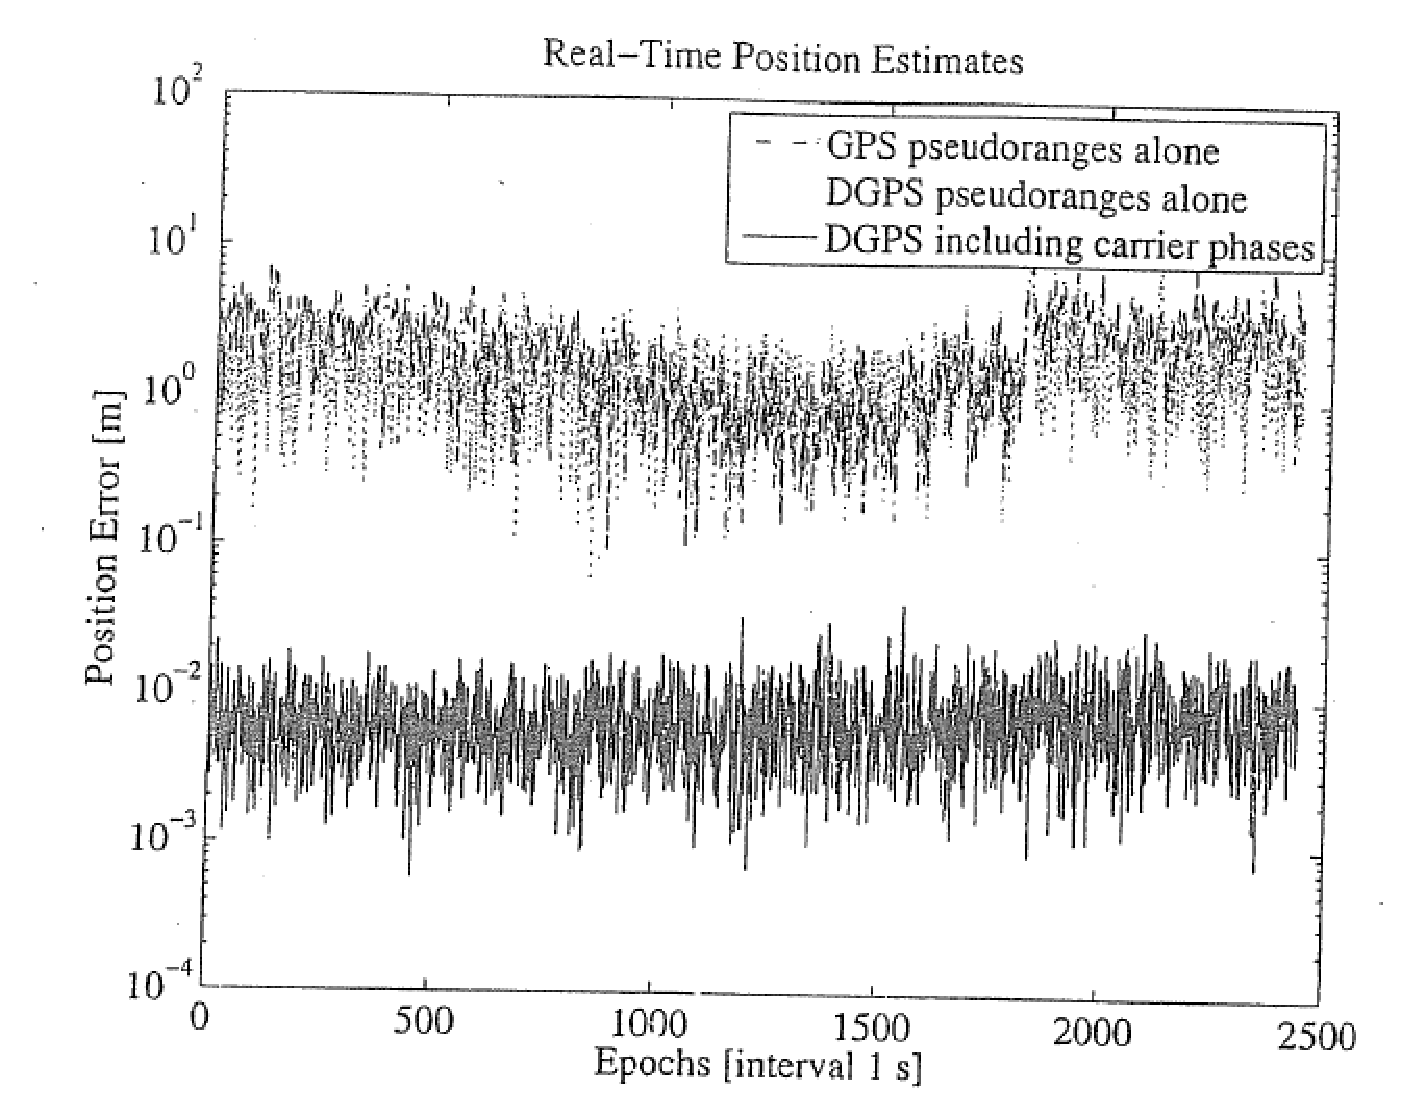
\includegraphics[width=0.4\linewidth]{TeX_files/Part03/chapter10/image/9-5}
	\caption{利用伪距观测值的单点定位和差分定位位置偏差为几米,加入载波相位观测值之后位置偏差降到厘米级水平甚至更低}
	\label{fig:9-5}
\end{figure}

这个代码是最接近实时RTK代码的,没有和接收机连接而是直接连接到笔记本电脑的com端口上。如果笔记本电脑的配置可以实现,那么用户可以设置端口使用I/O设备。对于一个端口来说下面的代码是从接收机的legacy.tex文件中读取数据流。

s = serial('COM2');

s.OutputBufferSize = 512;

s.InputBuffersize = 50000;

fopen(s);

s. BaudRate = 9600;

set(s,'TimeOut',1 );

s.RecordMode = 'index';

s.Record Detail = 'verbose';

s.RecordName = 'legacy.tex';

图10.5说明了GPS实时定位精度的两种水平,其位置误差在几米到几个厘米范围内变化。利用42分钟采样率为1s的观测值计算得到的位置误差被规范的画在图上。

L1伪距观测值的定位精度通常为几米。并发访问GPS主接收机(位置已知)的伪距观测值并不会显著减少误差,但它可能消除了一些位置上具有相同趋势的误差。

\begin{figure}
	\centering
	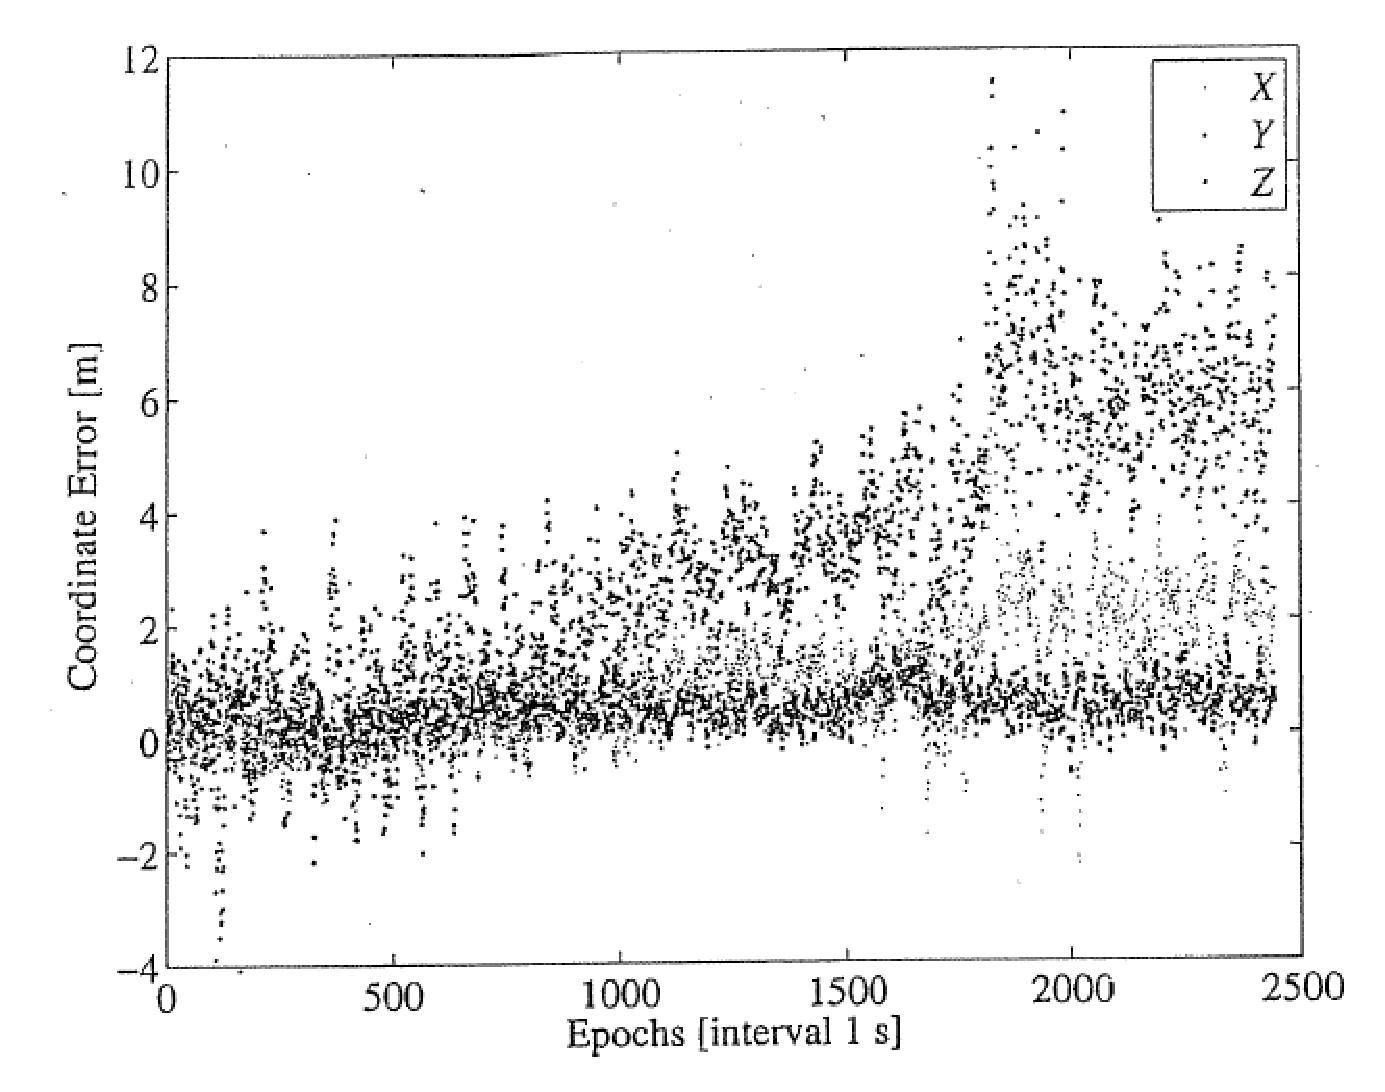
\includegraphics[width=0.4\linewidth]{TeX_files/Part03/chapter10/image/9-6}
	\caption{42分钟期间基准站坐标变化}
	\label{fig:9-6}
\end{figure}

充分利用伪距和载波相位观测值数据可以获得厘米级或者更好地定位精度。

图10.6 显示基准站在42分钟中仅利用伪距观测值获得的坐标变化,很明显X坐标、Y坐标的变化量小于Z坐标的变化(Aalborg,Denmark)。